\documentclass[11pt]{article}

\usepackage{fullpage} % Package to use full page
\usepackage{parskip} % Package to tweak paragraph skipping
\usepackage{tikz} % Package for drawing
\usepackage{amsmath}
\usepackage{hyperref}
\usepackage{graphicx}
\usepackage{authblk}
\usepackage[square,sort,comma,numbers]{natbib}
\usepackage{multirow}


%%%%%%%%%%%%%%%%%%%%%%%%%%%%%%%%%
\setlength{\textheight}{9in}
\setlength{\topmargin}{-0.600in}
\setlength{\headheight}{0.2in}
\setlength{\headsep}{0.250in}
\setlength{\footskip}{0.5in}
\flushbottom
\setlength{\textwidth}{6.5in}
\setlength{\oddsidemargin}{0in}
\setlength{\evensidemargin}{0in}
\setlength{\columnsep}{2pc}
\setlength{\parindent}{1em}
%%%%%%%%%%%%%%%%%%%%%%%%%%%%%%%%%

\title{Lending Club and Default Prediction Models}
\author{Kevin Reilly}
\author{John}
\affil{University of Utah -- Machine Learning}
\date{\today}

\begin{document}

\maketitle

\begin{abstract}
	The focus of this project was to evaluate various machine learning techniques in developing useful models for evaluating the importance of various attributes for loans in determining risk. 
Lending Club is a peer-to-peer lending application where users can request loans for various purposes and other users can fund these loans at a given rate and grade. This data is rich and noisy providing ample data to run against different loss methodologies. Our results indicate that logistic regression and neural nets perform fairly well against this particular dataset, while random forests overfit quickly and perceptron seemed too restrictive, indicating rigid linear models may not be ideal predictors. The trained models scored high sensitivities, and performed reasonably well for other metrics.
\end{abstract}

\section{Introduction}

\subsection{Objective}

The objective is to evaluate various methods for determining risk of default.  The methods we will evaluate are the State Vector Machines, Perceptrons, Random Forests, Logistic Regression, and Neural Nets. Several metrics will be used to evaluate against.  Since the data is already heavily weighed towards lower default rates (~20\%), simple precision metrics will not likely provide much insight into the models ability to correctly identify loans that are fully paid and loans that will default. 

\subsubsection{Metrics}
Sensitivity is the ratio of true positives against false negatives.  It measures the number of actual positive examples that were improperly classified as negative. 
\begin{equation}
sensitivity = \frac{TP}{TP + FN}
\end{equation}
Accuracy is the total correctly identified negatives and positives.  
\begin{equation}
accuracy = \frac{TN + TP}{N}
\end{equation}
Precision, in this case, measures the number of defaults that were modeled to be fully paid against the number correctly identified. 
\begin{equation}
precision = \frac{TP}{TP+FP}
\end{equation}
The F-score is the harmonic mean of the sensitivity and precision.  It can be used as a single measure of performance of the positive class. This will be the ultimate metric for which we will evaluate the total score for the test. 
\begin{equation}
F-Score = 2\frac{precision * recall}{precision + recall}
\end{equation}

\subsection{Data Set}

The dataset is provided by Lending Club on an ongoing basis for all the loans granted and denied on their application going as far back as 2007. The data is a set of all loans issued in the time period and their current status \cite{lendingclub}. Included are 145 columns relating to attributes of the loan itself, credit statistics, and Lending Club assigned variables  

\subsubsection{Data Cleaning}

Columns with text values were removed. Columns related to the loan status were also removed.  Every column less than half full were removed and rows with empty values were either filled with mean data or removed entirely depending on their likely effect on outcome.  

\subsubsection{Transform}

Categorical variables were replaced with their one-hot coded columns.  Zip and state columns were removed simply for their size when encoded. All other numerical variables were encoding around their unit norm. 

\subsection{Technical Process}

\paragraph{Data Attributes}
Newspaper3k, a python package, was used to extract the article data from raw html.  Golang was leveraged for its
concurrency capabilities to more effectively request the html data from the urls, given there were more than a quarter-million
incidents.

\paragraph{Preprocessing}
\cite{latexcompanion}
Further pre-processing of the set included removing stop words, puncuation, and numerics using the \texttt{gensim} python package. Some of this data is still relevant to the context of each article, however their importance for evaluation of this dataset was considered less critical.

\paragraph{Metrics}
\cite{knuthwebsite}
Vector representations of words for the corpus were generated using the GloVe model developed at Stanford.  The 300
dimensional vector representation appeared to provide the most differentiated analysis. The GloVe model assumes that
the meanings of words can be derived from the ratios of their occurence with other words, and the model here was developed
using a crawl of Wikipedia in 2014 and Gigaword 5. The Gigaword 5 corpus includes articles from various news organizations
over the span of five years and would contribute greatly to semantic word similarity in these vector representations.

\paragraph{Methods}
Random Forests, Perceptron, SVM, Neural Net


\section{Results}\label{sec:Results}

\subsection{Overall}

Our testing showed that nearly all of the tested models yielded similar results, achieving approximately 80\% accuracy in our best predictions, with F-metric over 89\%.

The best results were achieved by more complex models (particularly neural networks, which were tested under numerous parameters.) Logistic Regression also yielded strong results, prompting us to consider other statistical methods for future testing.

We observed that a single perceptron neuron was significantly inferior to all of the other included models, yielding over 5\% deterioration in accuracy metrics. We believe this is caused by the rigid linear classification of perceptron, which other models compensate for.

\subsubsection{Random Forests}

As expected, ensemble learning from decision trees quickly over-fits training data. The overall generalization to test data was not impacted heavily, however it seems that it may be difficult to improve this model with further modifications to the input data.

        \begin{center}
        \begin{tabular}{| c | c || c | c | c | c |}
        \hline
        Dataset & Label & Accuracy & F1 & Precision & Recall \\
        \hline \hline
         Training & Default         & 100.0\% & 100.0\% & 100.0\% & 100.0\% \\
         Training & Paid in Full    &       & 100.0\% & 100.0\% & 100.0\% \\
         \hline
         Test & Default             & 80.5\% & 12.7\% & 53.8\% & 7.2\% \\
         Test & Paid in Full        &       & 89.0\% & 81.2\% & 98.5\% \\
         \hline
        \end{tabular}
        \end{center}

\subsubsection{SVM}

The SVM model predicted as well as other models despite its linear nature, though did not quite match more expressive non-linear models.

        \begin{center}
        \begin{tabular}{| c | c || c | c | c | c |}
        \hline
        Dataset & Label & Accuracy & F1 & Precision & Recall \\
        \hline \hline
         Training & Default         & 80.1\% & 3.3\% & 50.5\% & 1.7\% \\
         Training & Paid in Full    &       & 88.9\% & 80.3\% & 99.6\% \\
         \hline
         Test & Default             & 80.3\% & 3.4\% & 48.7\% & 1.8\% \\
         Test & Paid in Full        &       & 89.0\% & 80.5\% & 99.5\% \\
         \hline
        \end{tabular}
        \end{center}

\subsubsection{Logistic Regression}

This model yielded the best overall results (though nearly identical to our final keras neural network implementation.)

        \begin{center}
        \begin{tabular}{| c | c || c | c | c | c |}
        \hline
        Dataset & Label & Accuracy & F1 & Precision & Recall \\
        \hline \hline
         Training & Default         & 80.3\% & 9.1\% & 55.3\% & 5.0\% \\
         Training & Paid in Full    &       & 88.9\% & 80.7\% & 99.0\% \\
         \hline
         Test & Default             & 80.5\% & 9.4\% & 55.1\% & 51.2\% \\
         Test & Paid in Full        &       & 89.1\% & 81.0\% & 99.0\% \\
         \hline
        \end{tabular}
        \end{center}

\subsection{Perceptron}

The single perceptron node was the worst predictor of the tested methods. It seems that this model may be too rigidly linear for the data.

        \begin{center}
        \begin{tabular}{| c | c || c | c | c | c |}
        \hline
        Dataset & Label & Accuracy & F1 & Precision & Recall \\
        \hline \hline
         Training & Default         & 74.2\% & 19.4\% & 25.6\% & 15.5\% \\
         Training & Paid in Full    &       & 84.6\% & 80.9\% & 88.8\% \\
         \hline
         Test & Default             & 74.4\% & 19.8\% & 26.0\% & 16.0\% \\
         Test & Paid in Full        &       & 84.8\% & 81.2\% & 88.8\% \\
         \hline
        \end{tabular}
        \end{center}

\subsubsection{Neural Net}

Of the numerous settings modeled in keras, we found that increasing the complexity of the model did not yield much improvement in our results. As such, we favored a somewhat simpler model of only $3 \times 20$ hidden features.

The following results were generated by the referenced model of 3 hidden layers, 20 nodes per layer:

        \begin{center}
        \begin{tabular}{| c | c || c | c | c | c |}
        \hline
        Dataset & Label & Accuracy & F1 & Precision & Recall \\
        \hline \hline
         Test & Paid in Full        & 80.4 & 89.0\% & 81.0\% & 98.7\% \\
         \hline
        \end{tabular}
        \end{center}

This figure demonstrates the change in outcome as we increased complexity of the network. It appears that overfitting begins to occur after a width of only 30 neurons with training error continuing to decrease but the generalization performance fluctuating.

\begin{figure}[h!]
	\centering
	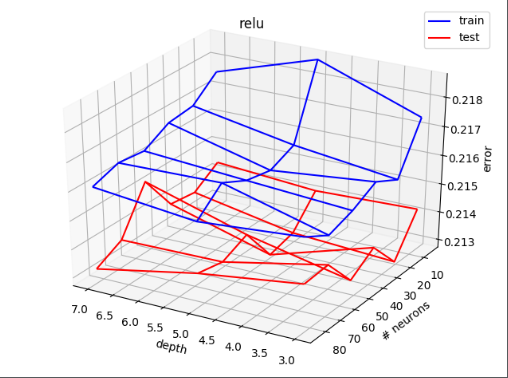
\includegraphics[width=10cm, height=7cm]{neural_nets.png}
	\caption{Train and Test Error for Various Architectures}
	\label{fig:neural_net}
\end{figure}


\section{Conclusions}

\subsubsection{Learnings}

\subsection{Future Steps}




\nocite{*}

\newpage{}

\bibliographystyle{ieeetr}

\bibliography{bibliography}

\end{document}